\begin{figure}[ht]
    \centering
    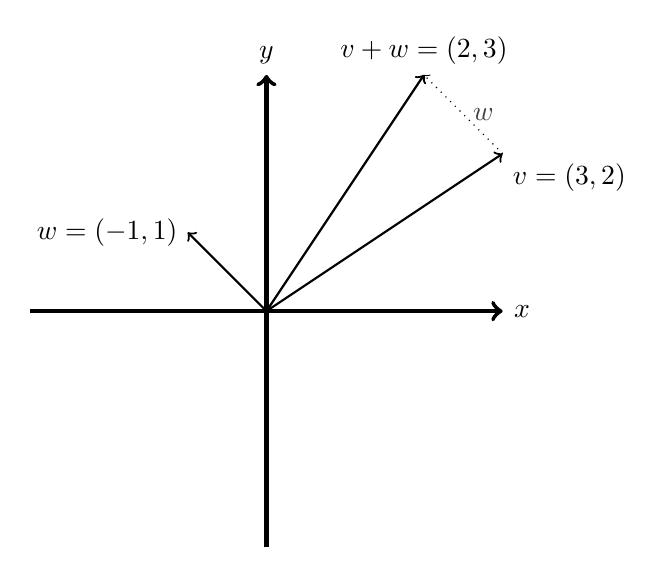
\begin{tikzpicture}
    \draw[->,ultra thick] (-3,0)--(3,0) node[right]{$x$};
    \draw[->,ultra thick] (0,-3)--(0,3) node[above]{$y$};
    % Vetor v=(3,2)
    \draw[->,thick] (0,0) -- (3,2) node[below right]{$v=(3,2)$};
    % Vetor w=(-1,1)
    \draw[->,thick] (0,0) -- (-1,1) node[left]{$w=(-1,1)$};
    % Vetor cópia w=(-1,1)
    \draw[->,dotted] (3,2) -- (2,3) node[midway, right, text=darkgray]{$w$};
    % Soma v+w
    \draw[->,thick] (0,0) -- (2,3) node[above, align=left]{$v+w=(2,3)$};
    \end{tikzpicture}
    \caption{Soma de vetores em $\mathbb R^2$.}
    \label{fig:soma-vetores}
\end{figure}
